\documentclass[a4paper,11pt,dvipdfmx]{jsarticle}

\usepackage{url}

% 数式
\usepackage{amsmath,amsfonts}
\usepackage{bm}

% 画像
\usepackage[dvipdfmx]{graphicx}
\usepackage{framed}

% 図形
\usepackage{tikz}
\usepackage{pgfplots}
\pgfplotsset{compat=1.18}
\usetikzlibrary{shapes.geometric}
\usetikzlibrary {shapes.misc}

% ソースコード
\usepackage{listings,jlisting,color}
\lstset{
language={Python},
backgroundcolor={\color[gray]{.85}},
basicstyle={\ttfamily},
identifierstyle={\small},
commentstyle={\small \color[rgb]{0,0.5,0}},
keywordstyle={\small\bfseries \color[rgb]{0.5,0,0.5}},
ndkeywordstyle={\small},
stringstyle={\small\ttfamily \color[rgb]{0,0,1}},
frame={tb},
breaklines=true,
columns=[l]{fullflexible},
numbers=left,
xrightmargin=0zw,
xleftmargin=3zw,
numberstyle={\scriptsize},
stepnumber=1,
numbersep=1zw,
lineskip=-0.5ex,
}
\renewcommand{\lstlistingname}{ソースコード}

\begin{document}
\begin{titlepage}
\noindent
\vspace{4cm}
\begin{center}
\begin{LARGE}
組込システムI \\
第4回  課題 \\
\vspace{8cm}
提出日  2025/05/15 \\
学籍番号  21T2166D \\
名前  渡辺 大樹 \\
\end{LARGE}
\end{center}
\end{titlepage}

\definecolor{shadecolor}{gray}{0.70}

\section{演習1 - 7セグメントLEDの真理値表}
\begin{shaded}
    \noindent
    \textbf{課題:} 7セグメントLED(C-551SRD)の各セグメントの接続状態を示す真理値表を作成しなさい。
\end{shaded}

以下が7セグメントLEDの各セグメントの接続状態を示す真理値表である。
\begin{center}
\begin{tabular}{|c|c|c|c|c|c|c|c|c|} 
\hline
\textbf{数字} & \textbf{A} & \textbf{B} & \textbf{C} & \textbf{D} & \textbf{E} & \textbf{F} & \textbf{G} \\
\hline
0 & H & H & H & H & H & H & L \\
1 & L & H & H & L & L & L & L \\
2 & H & H & L & H & H & L & H \\
3 & H & H & H & H & L & L & H \\
4 & L & H & H & L & L & H & H \\
5 & H & L & H & H & L & H & H \\
6 & H & L & H & H & H & H & H \\
7 & H & H & H & L & L & L & L \\
8 & H & H & H & H & H & H & H \\
9 & H & H & H & H & L & H & H \\
\hline
\end{tabular}
\end{center}

\section{演習3 - 7セグメントLEDルーレットの作成}
\begin{shaded}
    \noindent
    \textbf{課題1:} 7セグメントLEDに繰り返しランダムに数字(0~9)を表示し、スイッチにより任意のタイミングで表示を停止する回路、プログラムを作成しなさい。 \\
    \textbf{課題2:} この回路で、数字の表示、停止を30回以上行い、各数字の発生頻度をグラフで報告しなさい。

\end{shaded}

\subsection{課題1}

\subsubsection{回路}

以下、図\ref{exam4},\ref{kairozu}が7セグメントLEDに繰り返しランダムに数字(0~9)を表示し、スイッチにより任意のタイミングで表示を停止する回路,回路図である。
\begin{figure}[h]
\centering
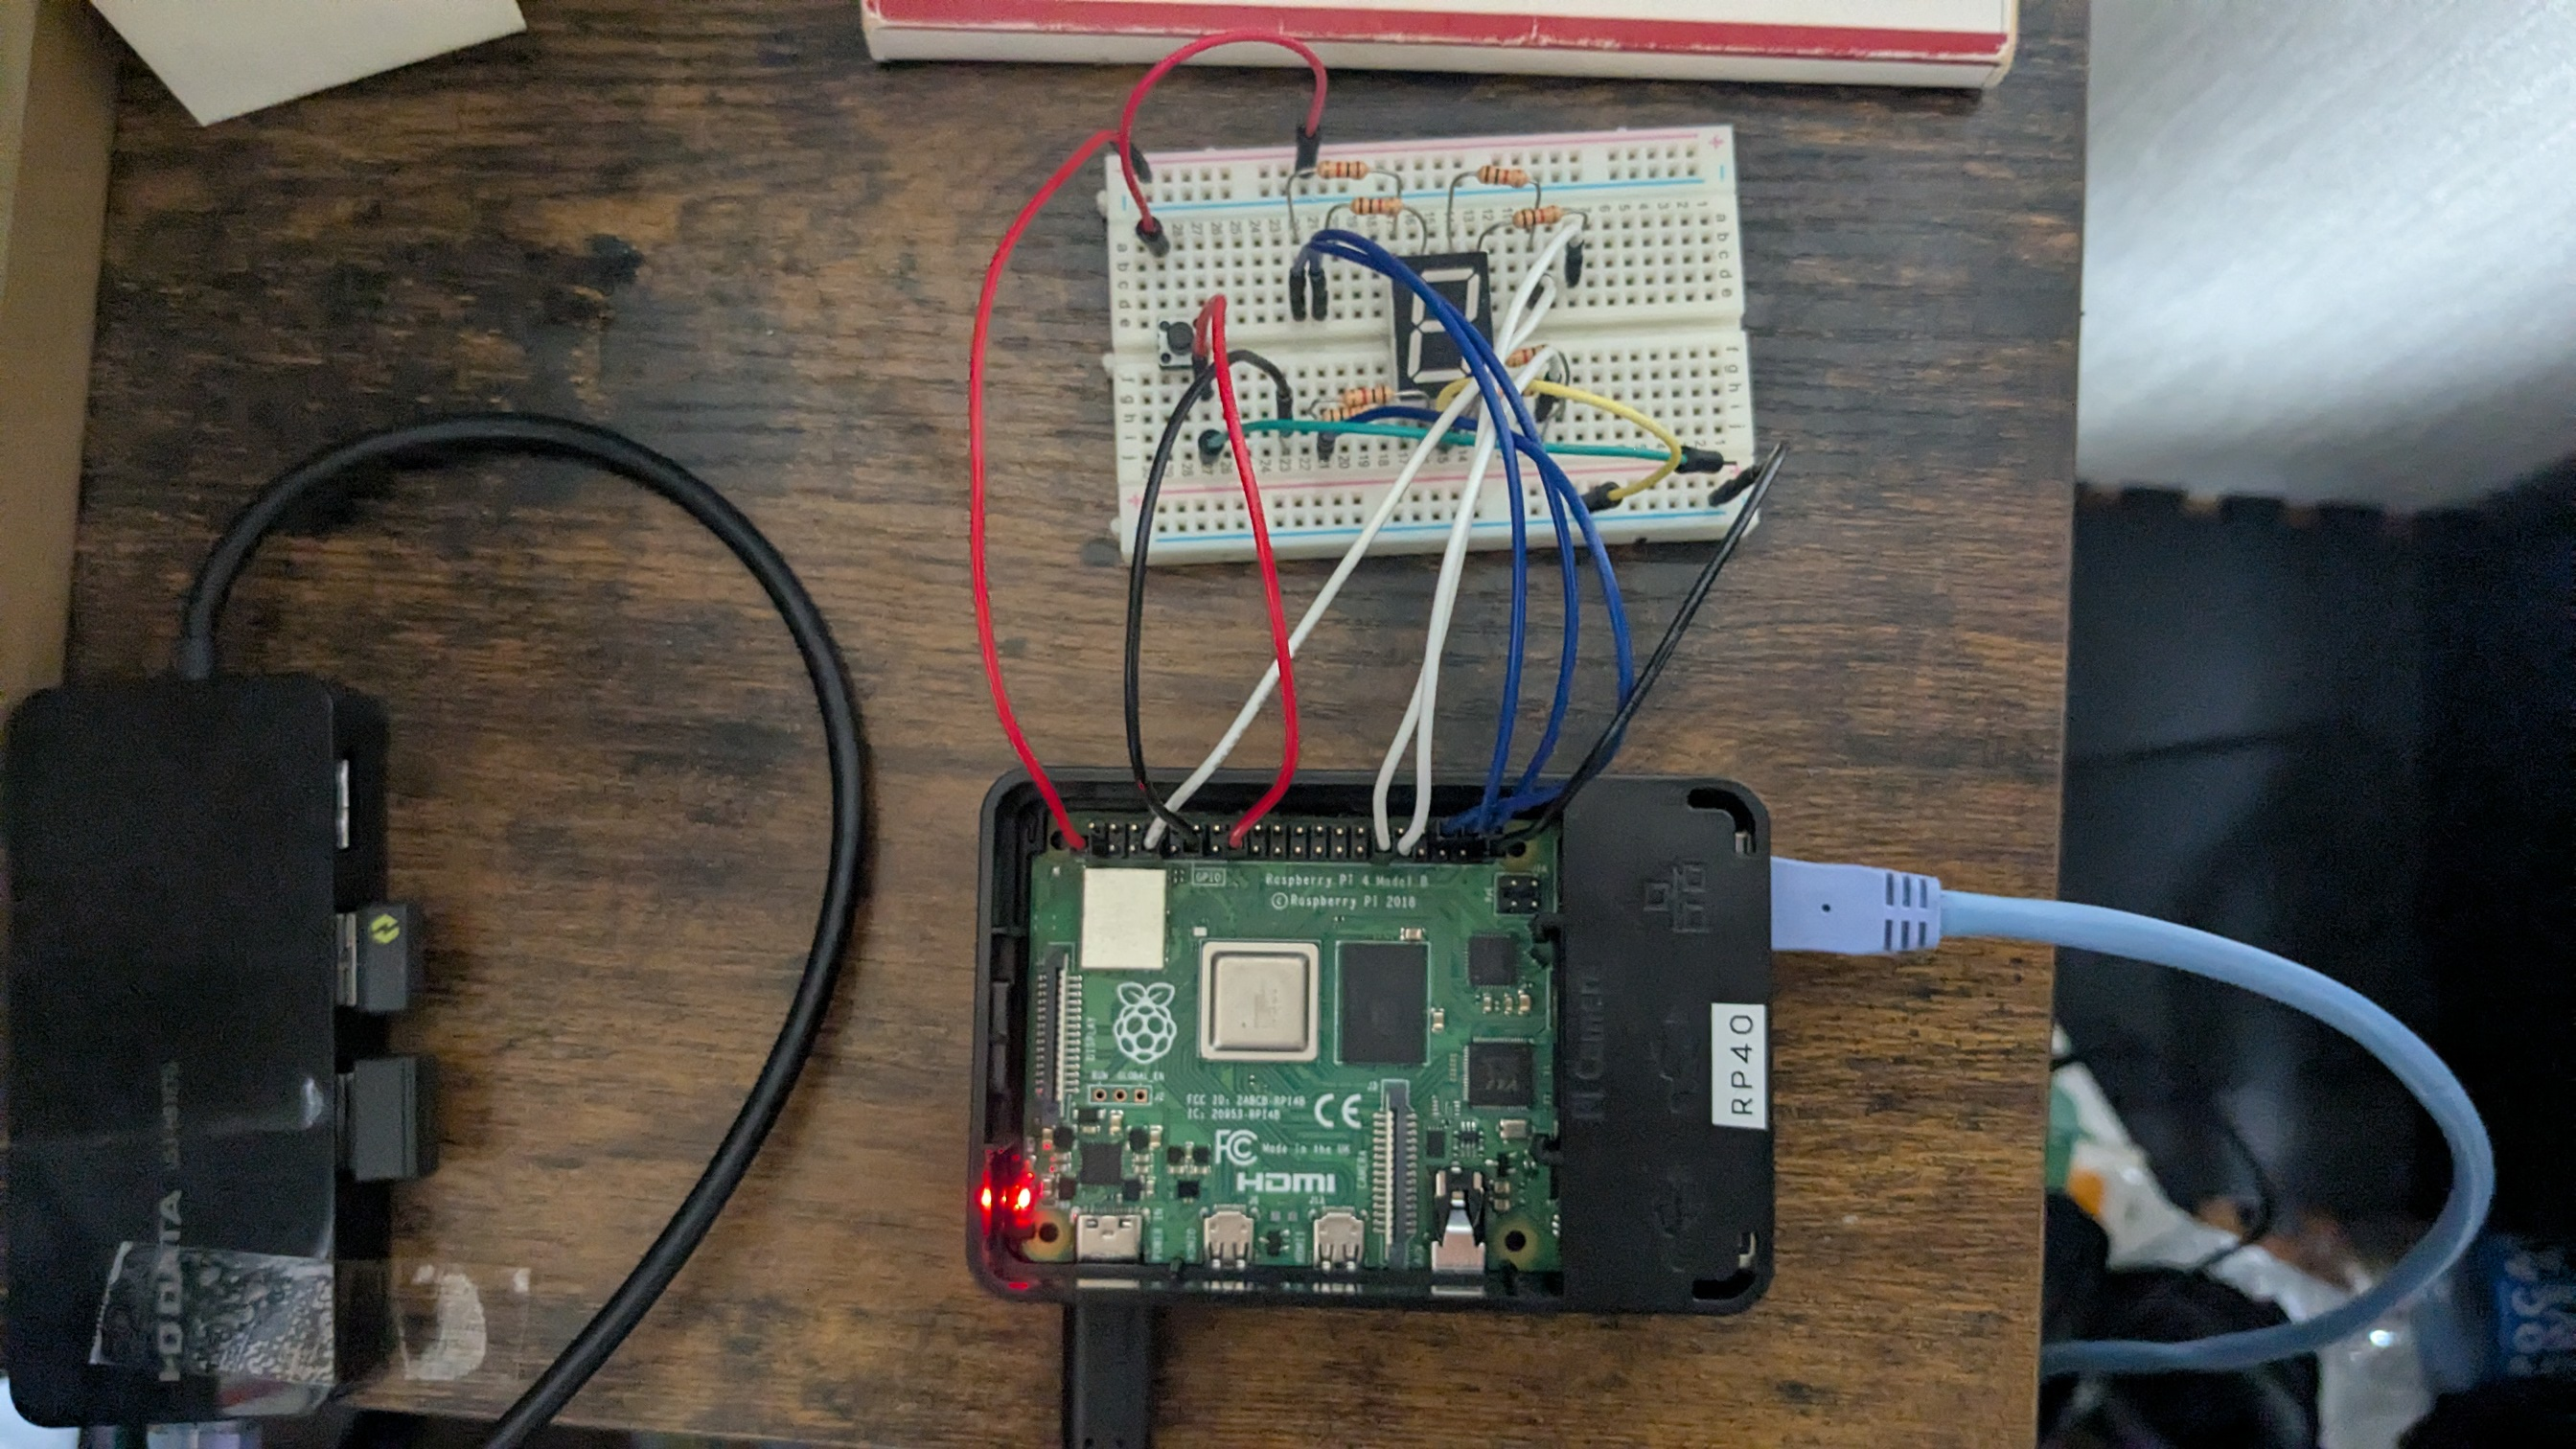
\includegraphics[width=100mm]{c:/Program_Code/LaTeX/BuiltIn/exam4/PXL_20250515_141152948.jpg}
\caption{7セグメントLEDルーレット}
\label{exam4}
\end{figure}

\begin{figure}[h]
\centering
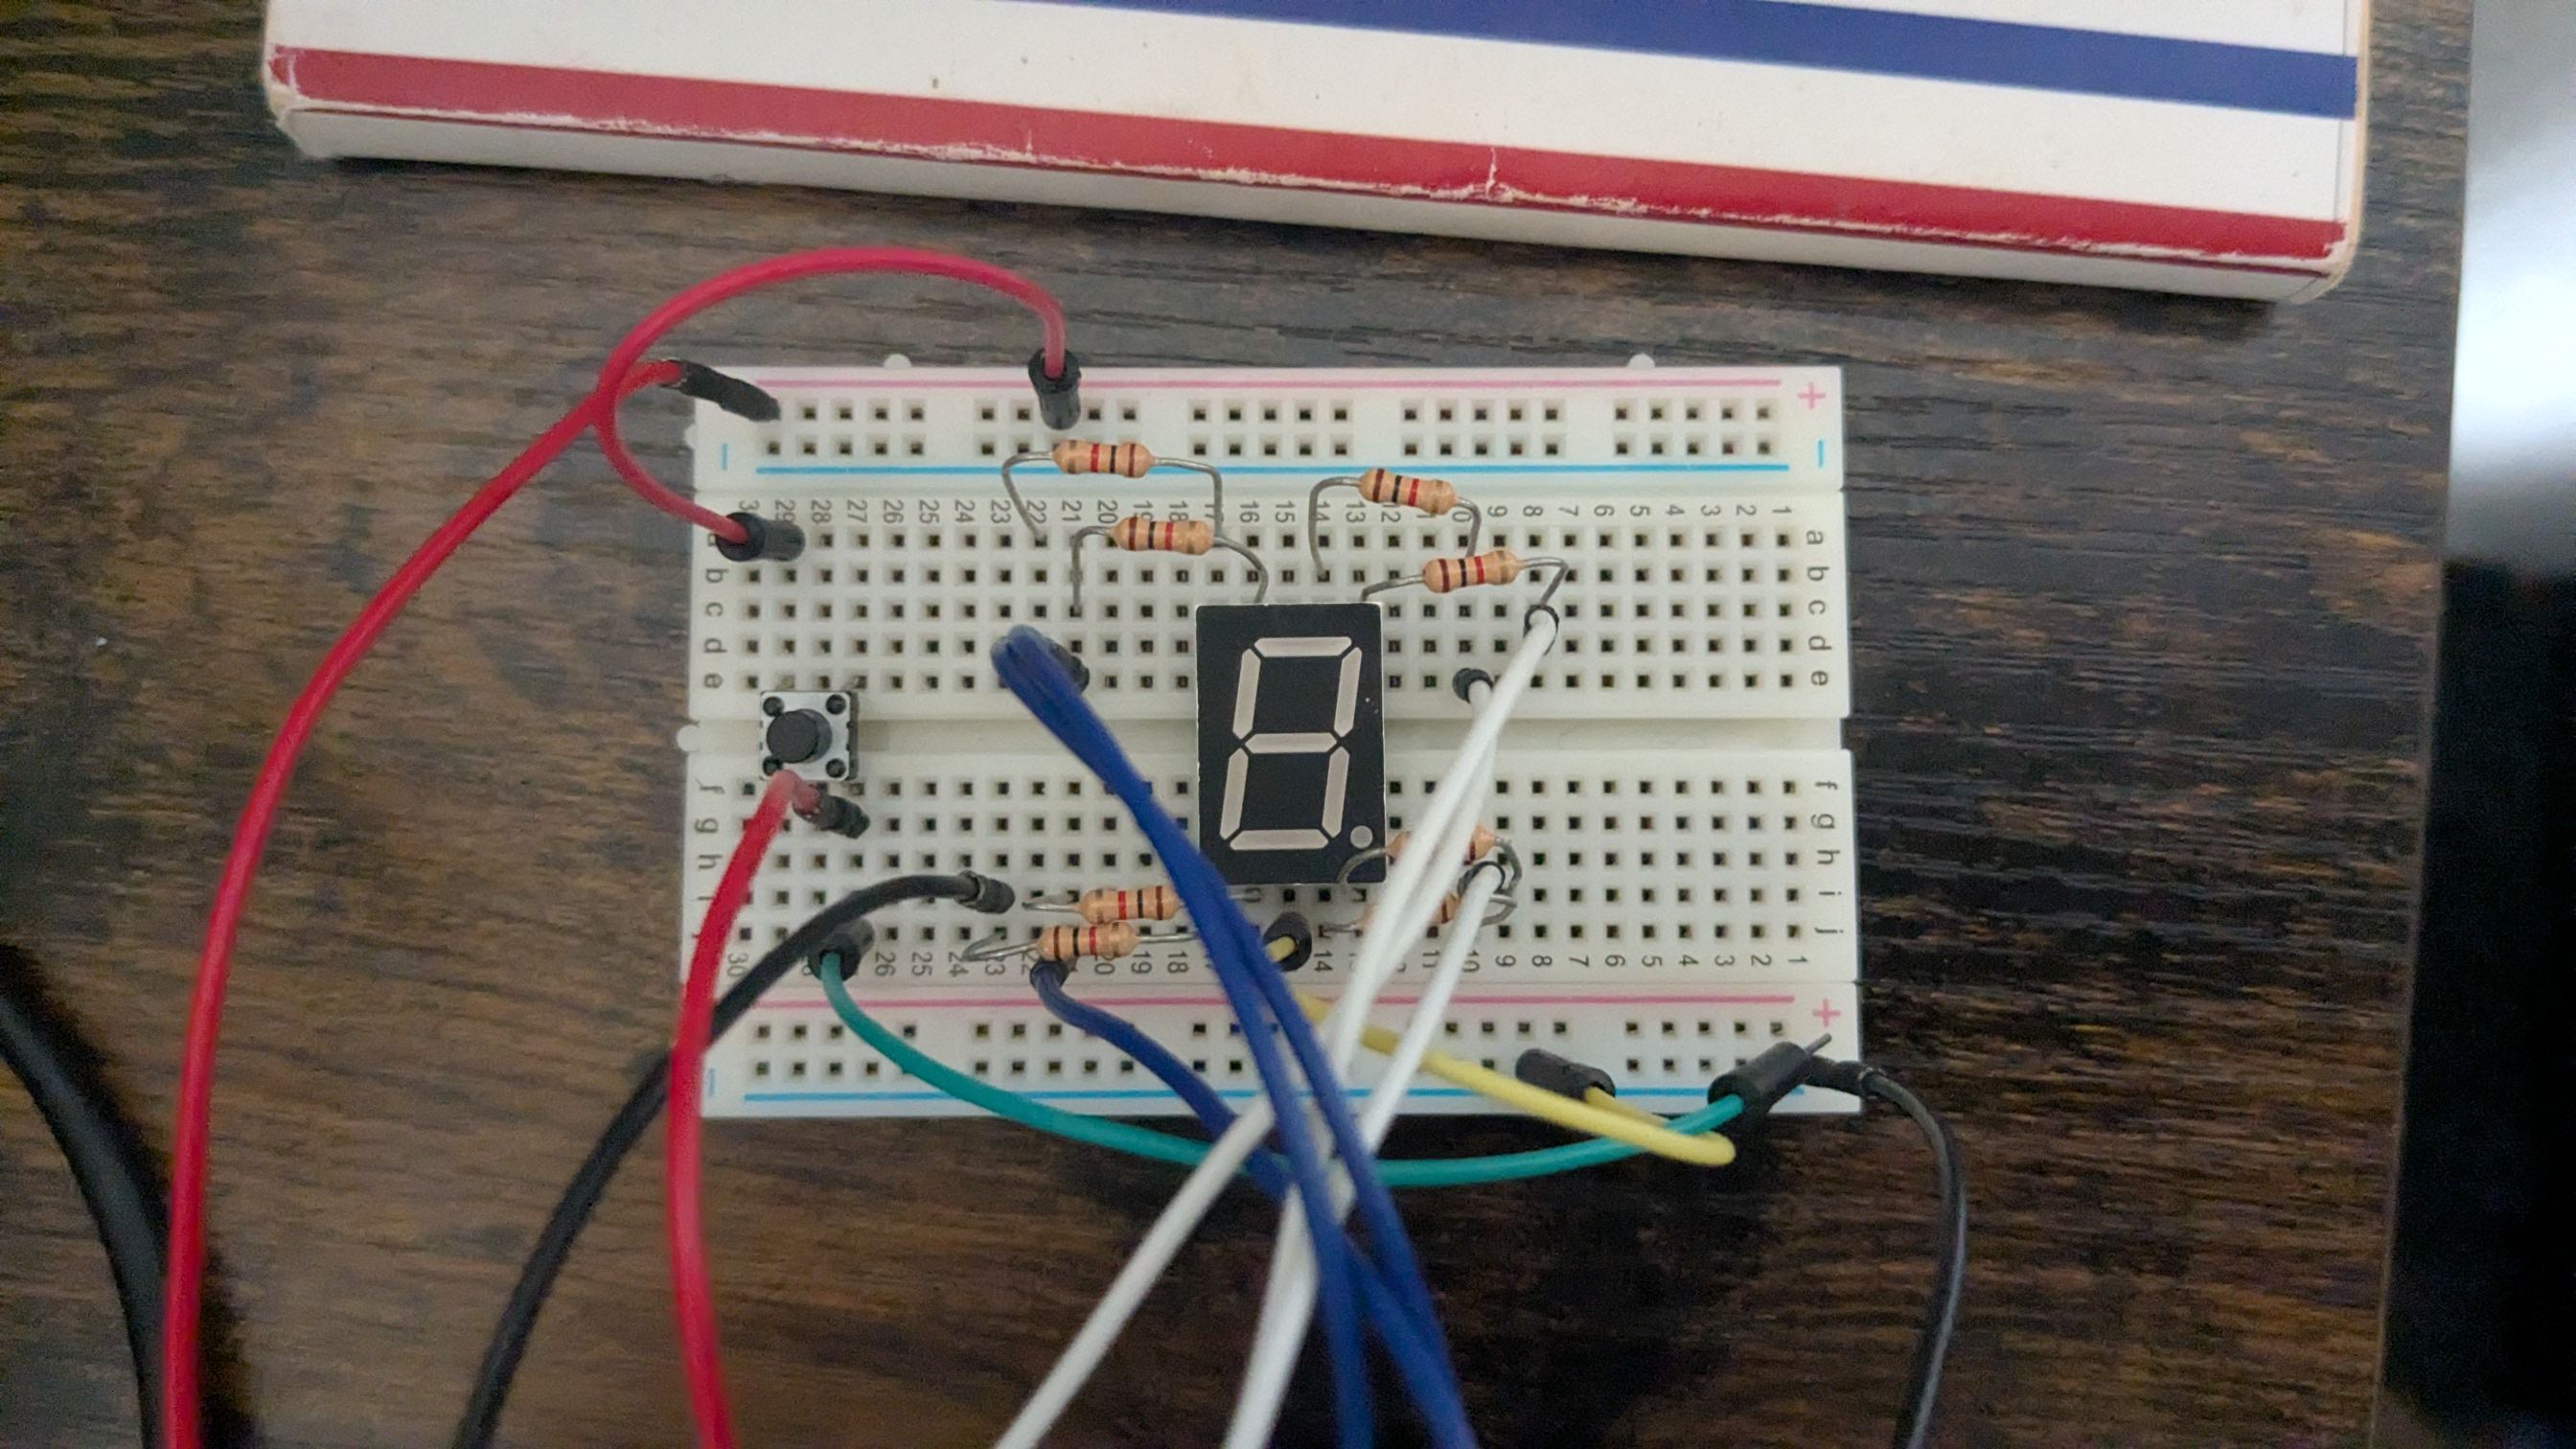
\includegraphics[width=100mm]{c:/Program_Code/LaTeX/BuiltIn/exam4/PXL_20250515_141203602.jpg}
\caption{7セグメントLEDルーレット回路図}
\label{kairozu}
\end{figure}

この回路は、セグメントの接続状態を示す真理値表を元に、7セグメントLEDの各セグメントに接続されたLEDを点灯させるための回路である。
また、スイッチを押すことで、7セグメントLEDに表示される数字を停止させることができる。

Raspberry Pi PicoのGPIOピンを使用して、7セグメントLEDの各セグメントを制御している。
接続先はそれぞれ
\begin{itemize}
    \item A: GPIO 4
    \item B: GPIO 5
    \item C: GPIO 6
    \item D: GPIO 16
    \item E: GPIO 17
    \item F: GPIO 20
    \item G: GPIO 21
    
\end{itemize}
となっている。
またタクトスイッチはGPIO 22に接続されている。

\subsubsection{使用部品}
\begin{itemize}
    \item Raspberry Pi 4 Model B
    \item 7セグメントLED(C-551SRD)
    \item タクトスイッチ
    \item 抵抗(1kΩ) * 8
    \item ブレッドボード
    \item ジャンパーワイヤー
\end{itemize}

\subsubsection{プログラム}
以下ソースコード\ref{exam4}が7セグメントLEDに繰り返しランダムに数字(0~9)を表示し、スイッチにより任意のタイミングで表示を停止するプログラムである。

このコードは7セグメントLEDに0から9までの数字をランダムに表示し、スイッチが押されたときに表示を停止する機能を実装している。主な特徴は以下の通りである:

\begin{itemize}
    \item プログラムは \texttt{RPi.GPIO} ライブラリを用いて Raspberry Pi の各種 GPIO ピンを制御している
    \item 7セグメントLEDの各セグメント(A~G)に対応する GPIO ピンを配列として定義し、効率的な制御を実現している
    \item 数字0~9の表示パターンを2次元配列として定義し、各セグメントの点灯・消灯状態を管理している
    \item スイッチ入力検出時には表示中の数字をカウントし、結果を保存する機能を実装している
    \item マルチスレッド処理により、LED表示制御とスイッチ入力の並列監視を実現している
    \item 表示中の数字をランダムに変更するため、\texttt{random} ライブラリを使用している
\end{itemize}

特に、カウント機能をつけたことで、容易に課題2であるカウントの実施が容易となっている。 \\
またshellのinputを監視することでstopを入力すると、ルーレットが止まるようにしている。

\subsection{課題2}
\begin{shaded}
    \noindent
    \textbf{課題2:} この回路で、数字の表示、停止を30回以上行い、各数字の発生頻度をグラフで報告しなさい。 

\end{shaded}
以下に課題2の結果を示す。\\
\begin{shaded}
\noindent
スイッチ押下回数: 45 \\
0: 4回 \\
1: 9回 \\
2: 3回 \\
3: 3回 \\
4: 2回 \\
5: 4回 \\
6: 5回 \\
7: 4回 \\
8: 6回 \\
9: 5回 
\end{shaded}

グラフで示すと以下の図\ref{graph}のようになる。
\begin{figure}[h]
\centering
\begin{tikzpicture}
\begin{axis}[
    ybar,
    bar width=0.6cm,
    width=12cm,
    height=8cm,
    xlabel={数字},
    ylabel={発生頻度},
    symbolic x coords={0,1,2,3,4,5,6,7,8,9},
    xtick=data,
    nodes near coords,
    ymin=0,
    ymax=10,
    enlarge x limits=0.15,
    grid=major,
    grid style={dashed,gray!30},
    title={7セグメントLEDルーレットの数字発生頻度 (n=45)},
]
\addplot coordinates {(0,4) (1,9) (2,3) (3,3) (4,2) (5,4) (6,5) (7,4) (8,6) (9,5)};
\end{axis}
\end{tikzpicture}
\caption{7セグメントLEDルーレットの発生頻度分布}
\label{graph}
\end{figure}

\subsection{考察}
7セグメントLEDルーレットの数字発生頻度を調査した結果、数字1が最も多く出現し、次いで数字8が多く出現した。
逆に数字4が最も少なく出現した。\\
また、全体的に数字の出現頻度は均等ではなく、特定の数字が多く出現する傾向が見られた。\\
今後の改善点としては、より均等な出現頻度を実現するために、乱数生成アルゴリズムの見直しや、スイッチ押下時の処理を改良することが考えられる。


\section{問い - A/D変換に関する「量子化誤差」について}
\begin{shaded}
    \noindent
    \textbf{問い:} A/D変換に関する「量子化誤差」について説明しなさい。
\end{shaded}
量子化誤差とは、アナログ信号をデジタル信号に変換する際に生じる誤差のことを指す。\\
A/D変換器は、連続的なアナログ信号を離散的なデジタル値に変換するが、この過程で信号の値を近似するため、元の信号と変換後の信号との間に誤差が生じる。\\
この誤差は、量子化ステップと呼ばれる最小の変化単位に依存し、量子化ステップが小さいほど誤差は小さくなる。\\
量子化誤差は、信号の精度や品質に影響を与えるため、特に音声や画像処理などの分野で重要な要素となる。\\
量子化誤差を最小限に抑えるためには、A/D変換器の分解能を高くすることや、適切なフィルタリング技術を使用することが重要である。\\
    

\lstinputlisting[caption={exam4.py}, label=exam4]{c:/Program_Code/Python/BuiltIn/exam4.py}

\end{document}